\documentclass[]{book}

%These tell TeX which packages to use.
\usepackage{array,epsfig}
\usepackage{amsmath}
\usepackage{amsfonts}
\usepackage{amssymb}
\usepackage{amsxtra}
\usepackage{amsthm}
\usepackage{mathrsfs}
\usepackage{color}

%Here I define some theorem styles and shortcut commands for symbols I use often
\theoremstyle{definition}
\newtheorem{defn}{Definition}
\newtheorem{thm}{Theorem}
\newtheorem{cor}{Corollary}
\newtheorem*{rmk}{Remark}
\newtheorem{lem}{Lemma}
\newtheorem*{joke}{Joke}
\newtheorem{ex}{Example}
\newtheorem*{soln}{Solution}
\newtheorem{prop}{Proposition}

\newcommand{\lra}{\longrightarrow}
\newcommand{\ra}{\rightarrow}
\newcommand{\surj}{\twoheadrightarrow}
\newcommand{\graph}{\mathrm{graph}}
\newcommand{\bb}[1]{\mathbb{#1}}
\newcommand{\Z}{\bb{Z}}
\newcommand{\Q}{\bb{Q}}
\newcommand{\R}{\bb{R}}
\newcommand{\C}{\bb{C}}
\newcommand{\N}{\bb{N}}
\newcommand{\M}{\mathbf{M}}
\newcommand{\m}{\mathbf{m}}
\newcommand{\MM}{\mathscr{M}}
\newcommand{\HH}{\mathscr{H}}
\newcommand{\Om}{\Omega}
\newcommand{\Ho}{\in\HH(\Om)}
\newcommand{\bd}{\partial}
\newcommand{\del}{\partial}
\newcommand{\bardel}{\overline\partial}
\newcommand{\textdf}[1]{\textbf{\textsf{#1}}\index{#1}}
\newcommand{\img}{\mathrm{img}}
\newcommand{\ip}[2]{\left\langle{#1},{#2}\right\rangle}
\newcommand{\inter}[1]{\mathrm{int}{#1}}
\newcommand{\exter}[1]{\mathrm{ext}{#1}}
\newcommand{\cl}[1]{\mathrm{cl}{#1}}
\newcommand{\ds}{\displaystyle}
\newcommand{\vol}{\mathrm{vol}}
\newcommand{\cnt}{\mathrm{ct}}
\newcommand{\osc}{\mathrm{osc}}
\newcommand{\LL}{\mathbf{L}}
\newcommand{\UU}{\mathbf{U}}
\newcommand{\support}{\mathrm{support}}
\newcommand{\AND}{\;\wedge\;}
\newcommand{\OR}{\;\vee\;}
\newcommand{\Oset}{\varnothing}
\newcommand{\st}{\ni}
\newcommand{\wh}{\widehat}

%Pagination stuff.
\setlength{\topmargin}{-.3 in}
\setlength{\oddsidemargin}{0in}
\setlength{\evensidemargin}{0in}
\setlength{\textheight}{9.in}
\setlength{\textwidth}{6.5in}
\pagestyle{empty}


\begin{document}

\begin{center}
{\Large Data 227 - Autumn 2023 \hspace{0.5cm} HW 2}\\
\textbf{Data Visualization and Communication - Trimble}\\ %You should put your name here
Due: Friday October 13, 2023  11:59pm   
\end{center}

\vspace{0.2 cm}

\subsection*{Homework 1, Hurricane tracks}

\begin{enumerate}
\item\label{hurricane}

The \texttt{storms.csv} file contains a subset of the NOAA Atlantic hurricane database best track data. The data includes the positions and attributes of named North Atlantic tropical storms from 1975-2020, measured every six hours during the lifetime of a storm. 

\begin{enumerate}
\item
Check the storage type of each variable and state whether it matches your expectations from reading the dataset documentation (i.e., are categorical variables saved as strings? are numerical variables saved as integers or floating points?). (1 pt)

\item Let’s take a closer look at a single storm. Choose a storm that has no missing values, and save a subset of the data belonging to that storm in a new dataframe. (Tropical storms live for a few weeks.  Don't treat storms with the same name in different years together.) (2 pts)
\item  Create a scatterplot comparing your storm’s maximum sustained windspeed (in knots) to its air pressure at the storm’s center (in millibars) for all six-hour measurements. Use different visual channels to also include information about the storm’s status and Saffir-Simpson storm category. How many attributes are displayed in your graph, and what channels are you using to encode them?  (note, hurricane/tropical storm status and wind speed, though they may be spread out into multiple columns, measure the same thing.)  (2 pts)
\item Describe the relationship between wind and pressure. Do the storms’ status and category seem to have any impact on this relationship? You may use external sources to answer second half of this question provided that you cite them. (2 pts)
\item Don’t forget that each storm was tracked over time and space. Create a scatterplot with latitude on the x-axis and longitude on the y-axis to recreate the storm’s path. In addition, encode information from tropicalstorm\_force\_diameter and hurricane\_force\_diameter–pay special attention to what Tufte has to say in this week’s reading. For an example, view my plot below. (3 pts)

\end{enumerate}

\begin{figure}
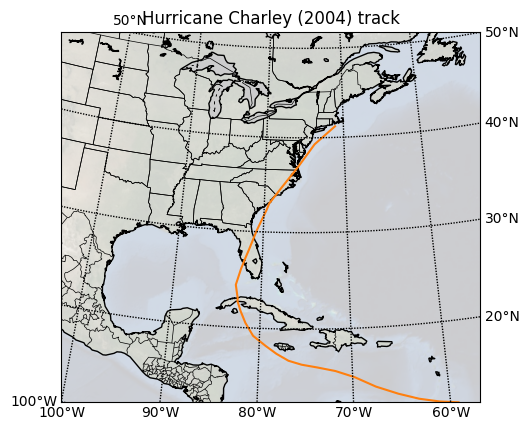
\includegraphics[width=12cm]{Charley.png}
\caption{Sample code to produce this map is provided}
\end{figure}

\item\label{bouy}

NOAA, the US federal government agency responsible for weather forecasting, maintains bouys in Lake Michigan with sensors that measure illumination, air temperature, water temperature, dewpoint, and other meteorological variables.

Station 45198, for instance, is near downtown Chicago and has data starting in 2021 to present (though some fields are missing for some dates).

\texttt{https://www.ndbc.noaa.gov/station\_history.php?station=45198}

Examine the data, find some fact about it, and design a data-rich visualization that communicates this fact.  

If you find the three years of history at this location limiting, you can obtain and plot data from other weather stations.


%\begin{soln}
%	% Put your answers here.
%\end{soln}


\end{enumerate}

\end{document}


